
\documentclass[a4paper,11pt]{article}
\usepackage{geometry}
\geometry{margin=2cm}
\usepackage{booktabs}
\usepackage{graphicx}
\usepackage{amsmath}
\usepackage{siunitx}
\usepackage{caption}
\usepackage{times}
\usepackage[utf8]{inputenc}
\usepackage{tocloft}
\usepackage{pdflscape} % Untuk mendukung landscape

\title{Spectral Simulation Report}
\author{Automated Analysis}
\date{\today}

\begin{document}

\maketitle
\tableofcontents
\clearpage

\section{Introduction}
This report presents the results of spectral simulations derived from HDF5 dataset analysis. Each sample includes a spectral plot displayed in a full horizontal page and a detailed table summarizing the initial composition, actual positions, total pixels, and signal-to-noise ratio (SNR), along with simulation parameters such as temperature and electron density.


\section{Sample: 10365}
\subsection{Simulation Parameters}
\begin{table}[h!]
    \centering
    \begin{tabular}{ll}
        \toprule
        \textbf{Parameter} & \textbf{Value} \\
        \midrule
        Temperature ($T$) & 7323 \,\si{K} \\
        Electron Density ($n_e$) & 5.86e+14 \,\si{cm^-3} \\
        Total Pixels & 4096 \\
        Signal-to-Noise Ratio (SNR) & 34.75 \\
        \bottomrule
    \end{tabular}
    \caption{Simulation parameters and additional metrics for sample 10365.}
    \label{tab:params_10365}
\end{table}

\subsection{Composition Analysis}
\begin{table}[h!]
    \centering
    \begin{tabular}{lcc}
        \toprule
        \textbf{Element} & \textbf{Initial Composition (\%)} & \textbf{Actual Positions} \\
        \midrule
        Al & 0.00 & 0.0 \\
        Ar & 0.84 & 657.0 \\
        C & 11.91 & 226.0 \\
        Ca & 5.45 & 150.0 \\
        Cl & 15.37 & 12.0 \\
        Co & 11.62 & 1402.0 \\
        Cr & 2.75 & 397.0 \\
        Fe & 4.98 & 2696.0 \\
        Mg & 13.72 & 316.0 \\
        Mn & 0.00 & 0.0 \\
        N & 0.00 & 0.0 \\
        Na & 9.11 & 322.0 \\
        Ni & 12.28 & 478.0 \\
        O & 0.00 & 0.0 \\
        S & 3.79 & 30.0 \\
        Si & 8.17 & 220.0 \\
        Ti & 0.00 & 0.0 \\
        background & N/A & 698.0 \\

        \midrule
        \textbf{Total Positions} & & 7604.0 \\
        \bottomrule
    \end{tabular}
    \caption{Composition analysis for sample 10365.}
    \label{tab:comp_10365}
\end{table}

\subsection{Spectral Plot}
\begin{figure}[p]
    \begin{landscape}
        \centering
        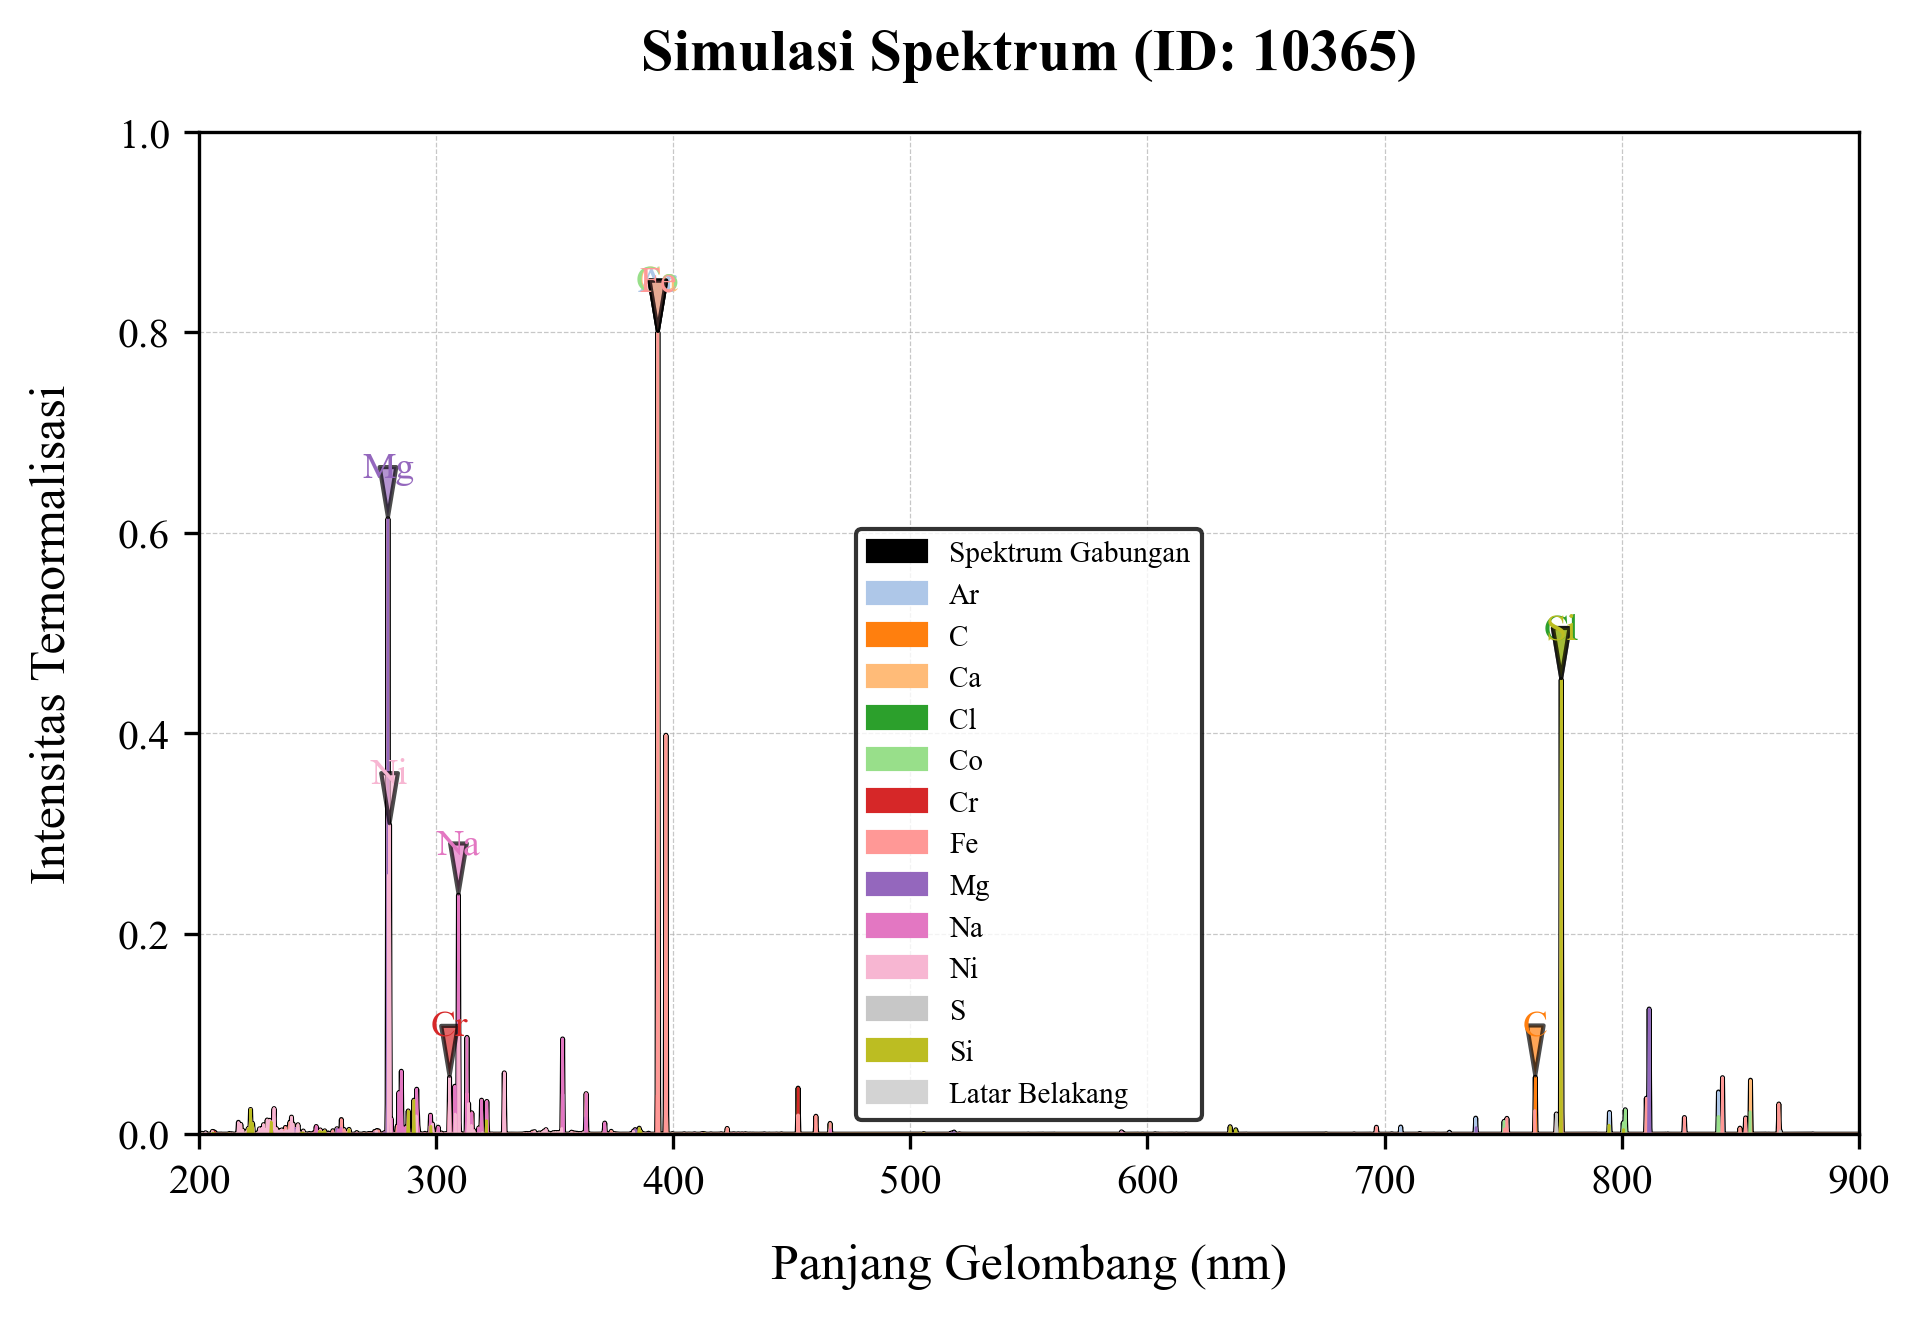
\includegraphics[width=1.2\textwidth, angle=90]{spectrum_10365.png}
        \caption{Spectral simulation plot for sample 10365 in full horizontal layout.}
        \label{fig:spectrum_10365}
    \end{landscape}
\end{figure}

\clearpage

\section{Sample: 13810}
\subsection{Simulation Parameters}
\begin{table}[h!]
    \centering
    \begin{tabular}{ll}
        \toprule
        \textbf{Parameter} & \textbf{Value} \\
        \midrule
        Temperature ($T$) & 8636 \,\si{K} \\
        Electron Density ($n_e$) & 3.27e+17 \,\si{cm^-3} \\
        Total Pixels & 4096 \\
        Signal-to-Noise Ratio (SNR) & 31.14 \\
        \bottomrule
    \end{tabular}
    \caption{Simulation parameters and additional metrics for sample 13810.}
    \label{tab:params_13810}
\end{table}

\subsection{Composition Analysis}
\begin{table}[h!]
    \centering
    \begin{tabular}{lcc}
        \toprule
        \textbf{Element} & \textbf{Initial Composition (\%)} & \textbf{Actual Positions} \\
        \midrule
        Al & 15.00 & 425.0 \\
        Ar & 0.00 & 0.0 \\
        C & 0.00 & 0.0 \\
        Ca & 5.95 & 150.0 \\
        Cl & 11.02 & 12.0 \\
        Co & 0.00 & 0.0 \\
        Cr & 9.42 & 397.0 \\
        Fe & 0.00 & 0.0 \\
        Mg & 6.49 & 341.0 \\
        Mn & 1.22 & 706.0 \\
        N & 0.00 & 0.0 \\
        Na & 14.91 & 330.0 \\
        Ni & 8.67 & 478.0 \\
        O & 16.69 & 168.0 \\
        S & 0.85 & 25.0 \\
        Si & 9.77 & 218.0 \\
        Ti & 0.00 & 0.0 \\
        background & N/A & 1932.0 \\

        \midrule
        \textbf{Total Positions} & & 5182.0 \\
        \bottomrule
    \end{tabular}
    \caption{Composition analysis for sample 13810.}
    \label{tab:comp_13810}
\end{table}

\subsection{Spectral Plot}
\begin{figure}[p]
    \begin{landscape}
        \centering
        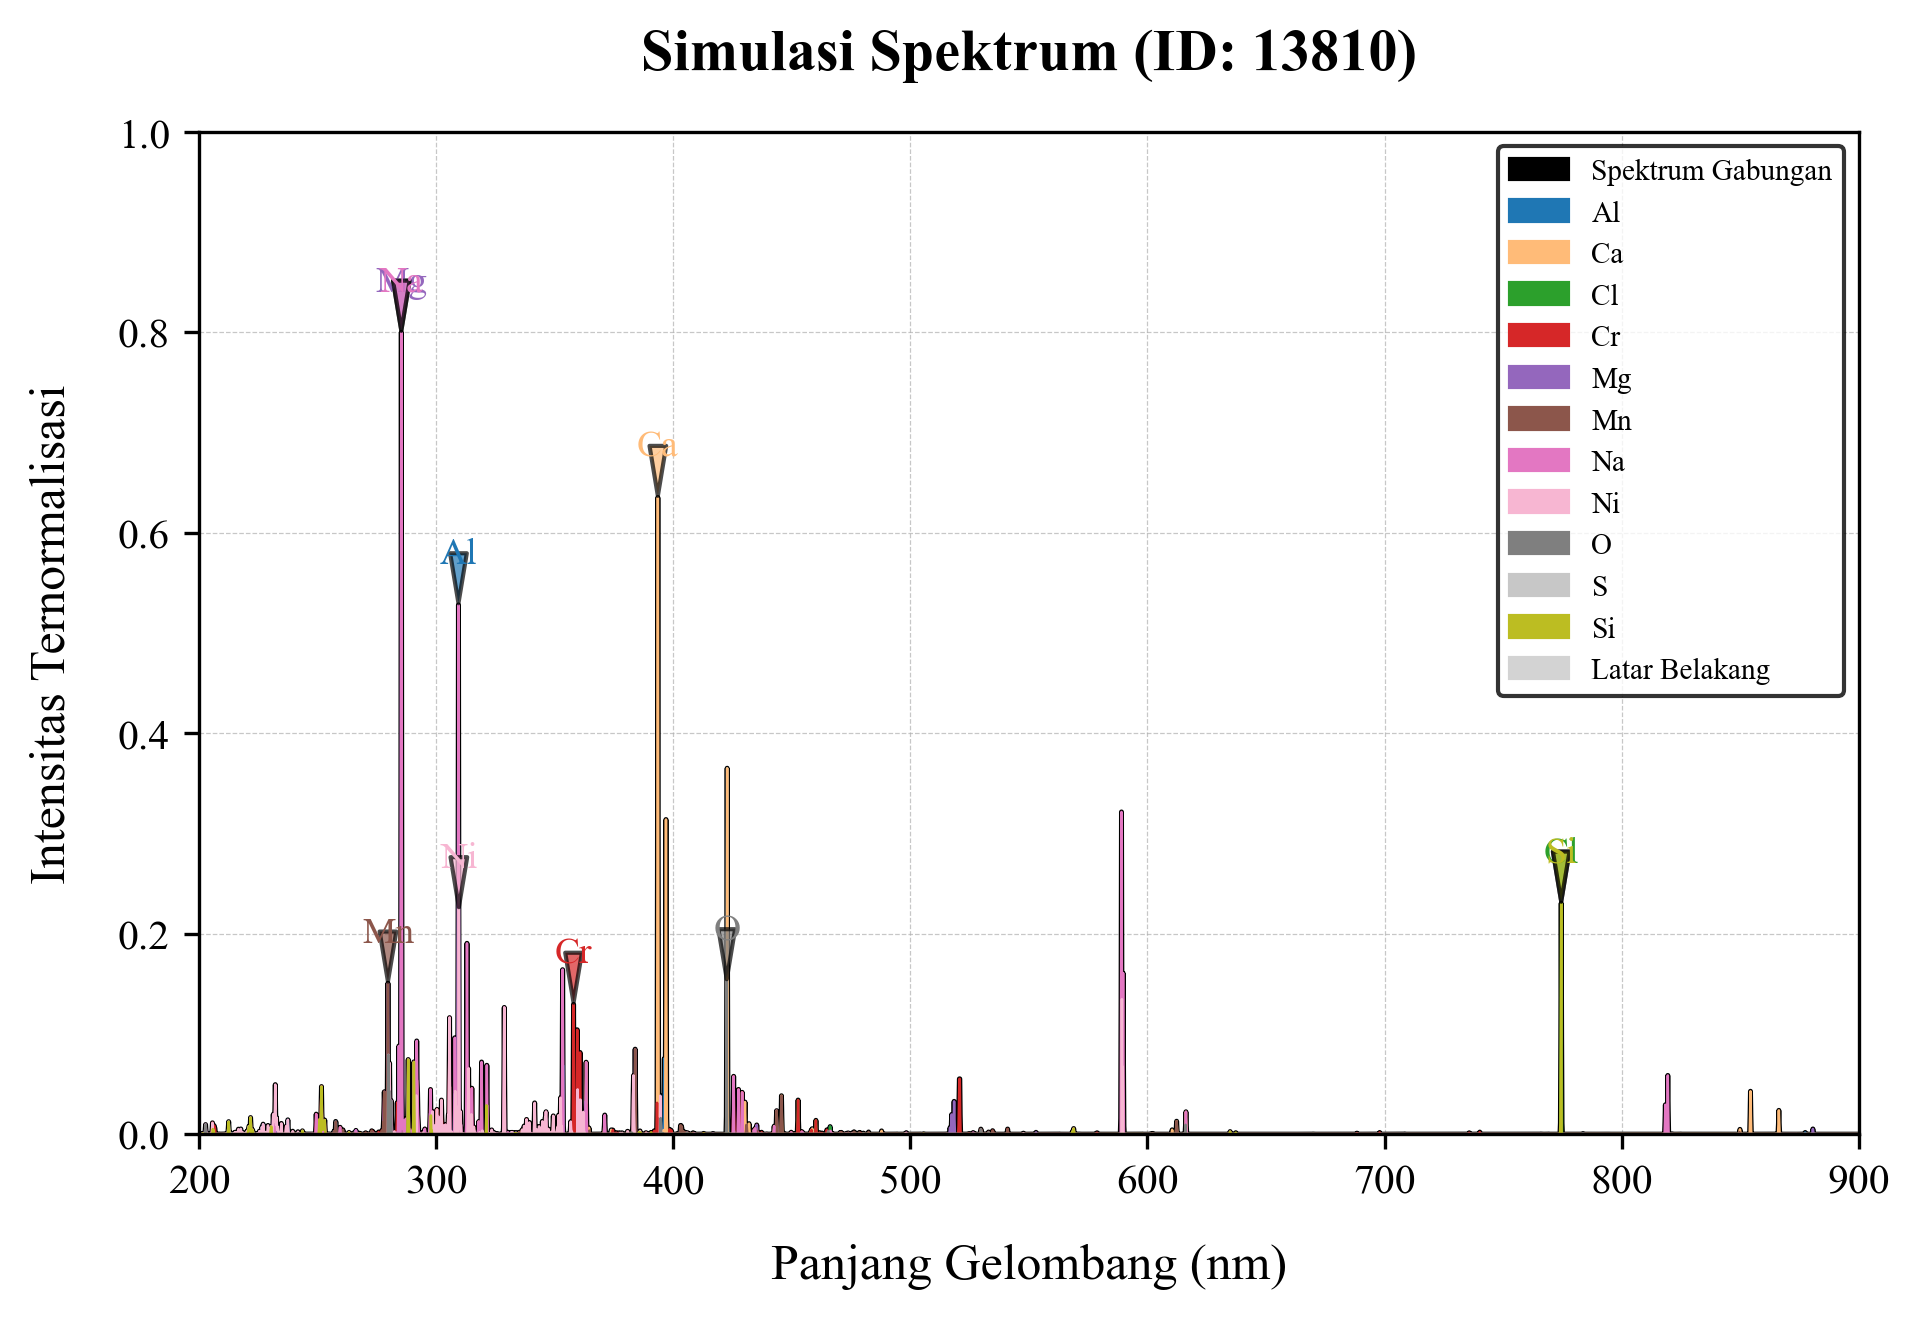
\includegraphics[width=1.2\textwidth, angle=90]{spectrum_13810.png}
        \caption{Spectral simulation plot for sample 13810 in full horizontal layout.}
        \label{fig:spectrum_13810}
    \end{landscape}
\end{figure}

\clearpage

\section{Sample: 193}
\subsection{Simulation Parameters}
\begin{table}[h!]
    \centering
    \begin{tabular}{ll}
        \toprule
        \textbf{Parameter} & \textbf{Value} \\
        \midrule
        Temperature ($T$) & 5909 \,\si{K} \\
        Electron Density ($n_e$) & 5.34e+14 \,\si{cm^-3} \\
        Total Pixels & 4096 \\
        Signal-to-Noise Ratio (SNR) & 37.52 \\
        \bottomrule
    \end{tabular}
    \caption{Simulation parameters and additional metrics for sample 193.}
    \label{tab:params_193}
\end{table}

\subsection{Composition Analysis}
\begin{table}[h!]
    \centering
    \begin{tabular}{lcc}
        \toprule
        \textbf{Element} & \textbf{Initial Composition (\%)} & \textbf{Actual Positions} \\
        \midrule
        Al & 4.88 & 140.0 \\
        Ar & 8.57 & 355.0 \\
        C & 9.52 & 167.0 \\
        Ca & 4.64 & 150.0 \\
        Cl & 6.81 & 12.0 \\
        Co & 3.67 & 862.0 \\
        Cr & 6.37 & 397.0 \\
        Fe & 0.00 & 0.0 \\
        Mg & 3.93 & 160.0 \\
        Mn & 9.55 & 673.0 \\
        N & 4.90 & 396.0 \\
        Na & 5.52 & 322.0 \\
        Ni & 0.30 & 478.0 \\
        O & 2.06 & 8.0 \\
        S & 9.80 & 25.0 \\
        Si & 11.34 & 205.0 \\
        Ti & 8.16 & 1181.0 \\
        background & N/A & 1210.0 \\

        \midrule
        \textbf{Total Positions} & & 6741.0 \\
        \bottomrule
    \end{tabular}
    \caption{Composition analysis for sample 193.}
    \label{tab:comp_193}
\end{table}

\subsection{Spectral Plot}
\begin{figure}[p]
    \begin{landscape}
        \centering
        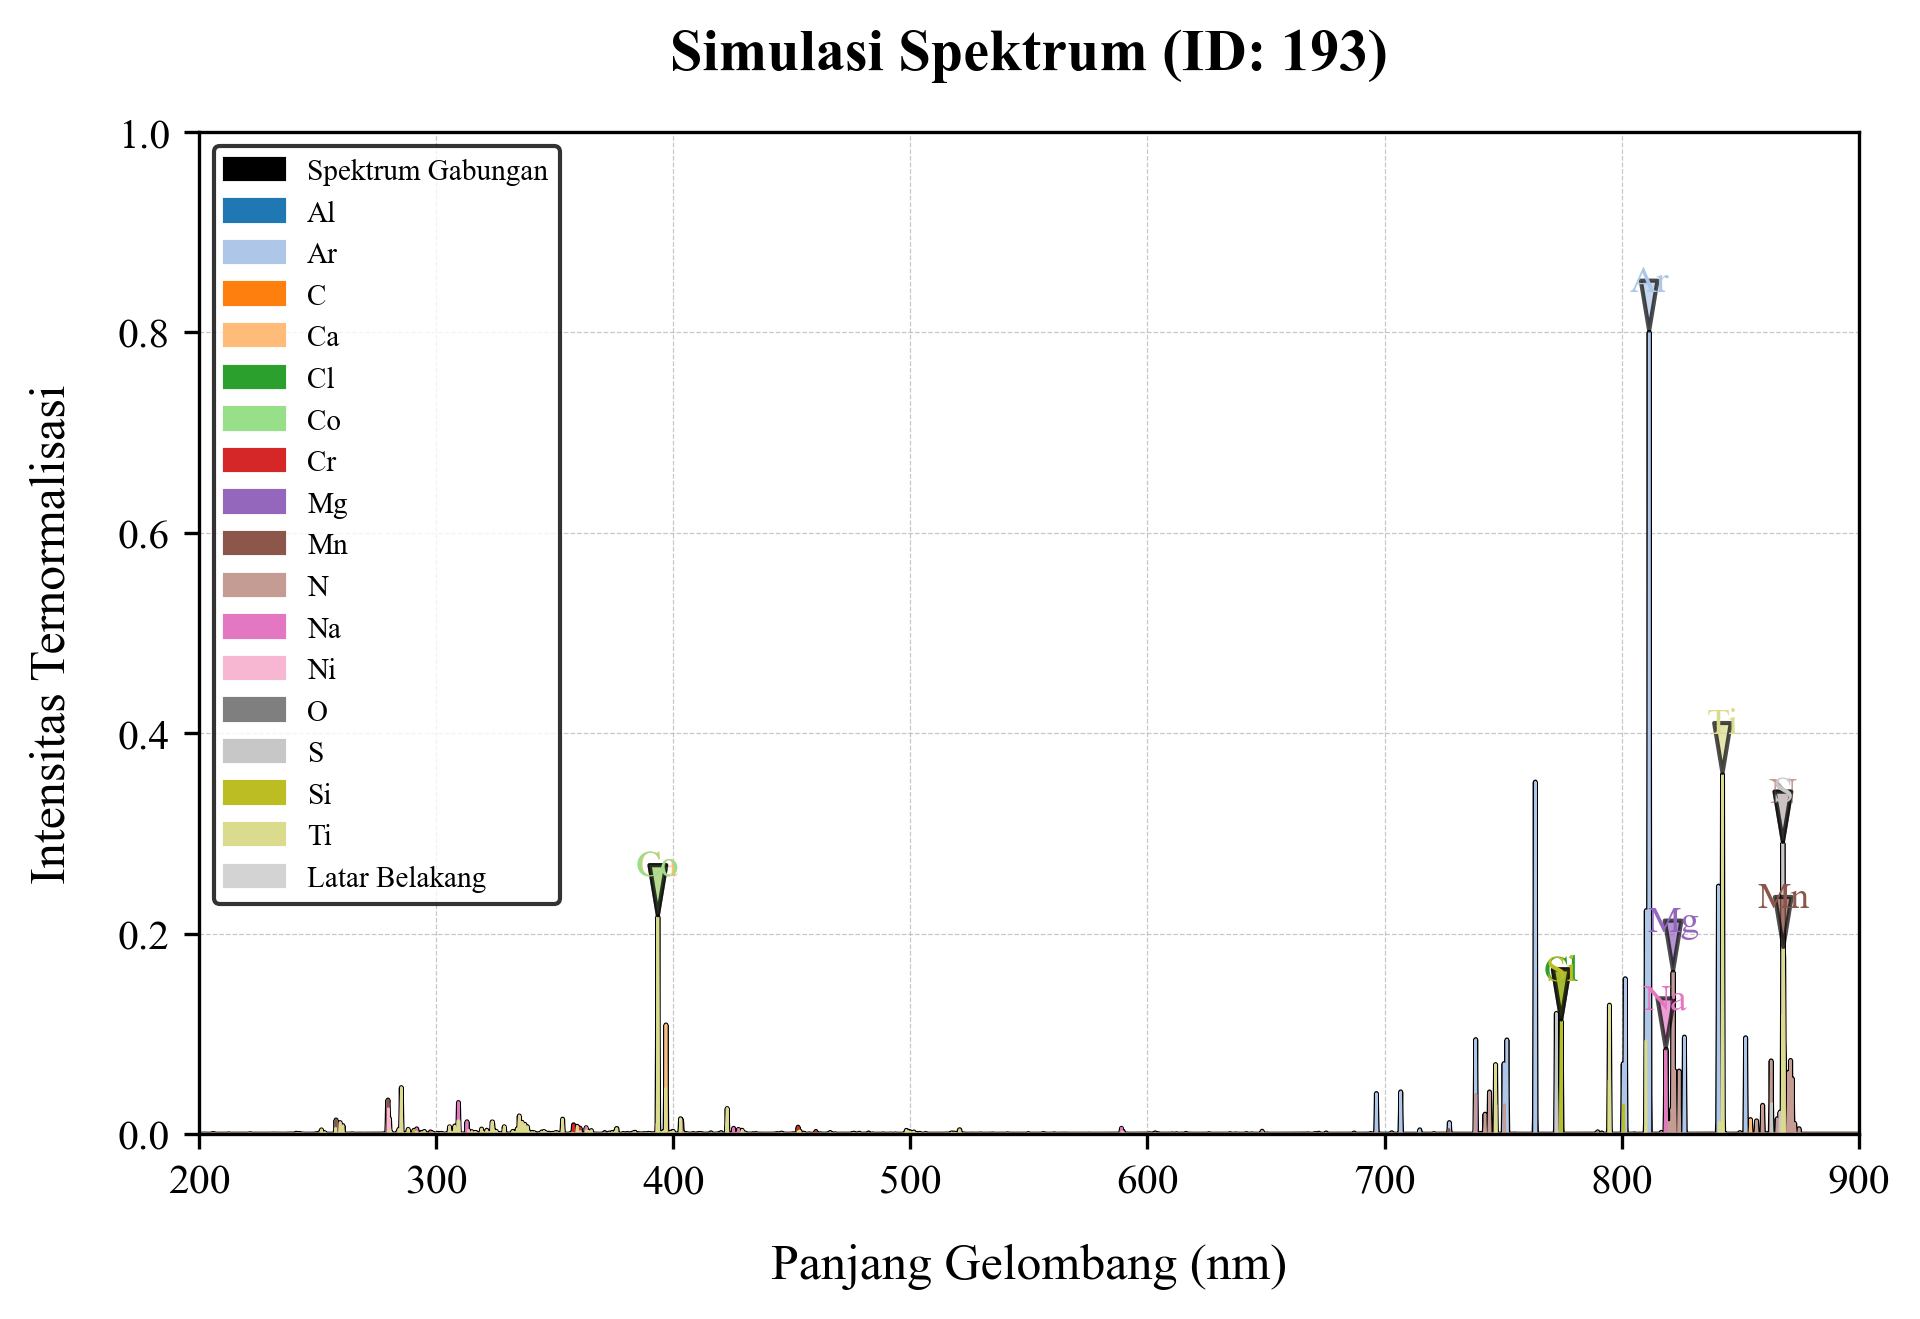
\includegraphics[width=1.2\textwidth, angle=90]{spectrum_193.png}
        \caption{Spectral simulation plot for sample 193 in full horizontal layout.}
        \label{fig:spectrum_193}
    \end{landscape}
\end{figure}

\clearpage

\section{Sample: 674}
\subsection{Simulation Parameters}
\begin{table}[h!]
    \centering
    \begin{tabular}{ll}
        \toprule
        \textbf{Parameter} & \textbf{Value} \\
        \midrule
        Temperature ($T$) & 12576 \,\si{K} \\
        Electron Density ($n_e$) & 2.60e+15 \,\si{cm^-3} \\
        Total Pixels & 4096 \\
        Signal-to-Noise Ratio (SNR) & 41.82 \\
        \bottomrule
    \end{tabular}
    \caption{Simulation parameters and additional metrics for sample 674.}
    \label{tab:params_674}
\end{table}

\subsection{Composition Analysis}
\begin{table}[h!]
    \centering
    \begin{tabular}{lcc}
        \toprule
        \textbf{Element} & \textbf{Initial Composition (\%)} & \textbf{Actual Positions} \\
        \midrule
        Al & 6.23 & 462.0 \\
        Ar & 1.46 & 727.0 \\
        C & 11.79 & 688.0 \\
        Ca & 16.90 & 150.0 \\
        Cl & 7.05 & 35.0 \\
        Co & 0.00 & 0.0 \\
        Cr & 7.85 & 397.0 \\
        Fe & 0.00 & 0.0 \\
        Mg & 7.85 & 352.0 \\
        Mn & 2.19 & 706.0 \\
        N & 0.00 & 0.0 \\
        Na & 6.67 & 322.0 \\
        Ni & 10.93 & 478.0 \\
        O & 3.82 & 255.0 \\
        S & 4.90 & 226.0 \\
        Si & 0.85 & 219.0 \\
        Ti & 11.51 & 1189.0 \\
        background & N/A & 1053.0 \\

        \midrule
        \textbf{Total Positions} & & 7259.0 \\
        \bottomrule
    \end{tabular}
    \caption{Composition analysis for sample 674.}
    \label{tab:comp_674}
\end{table}

\subsection{Spectral Plot}
\begin{figure}[p]
    \begin{landscape}
        \centering
        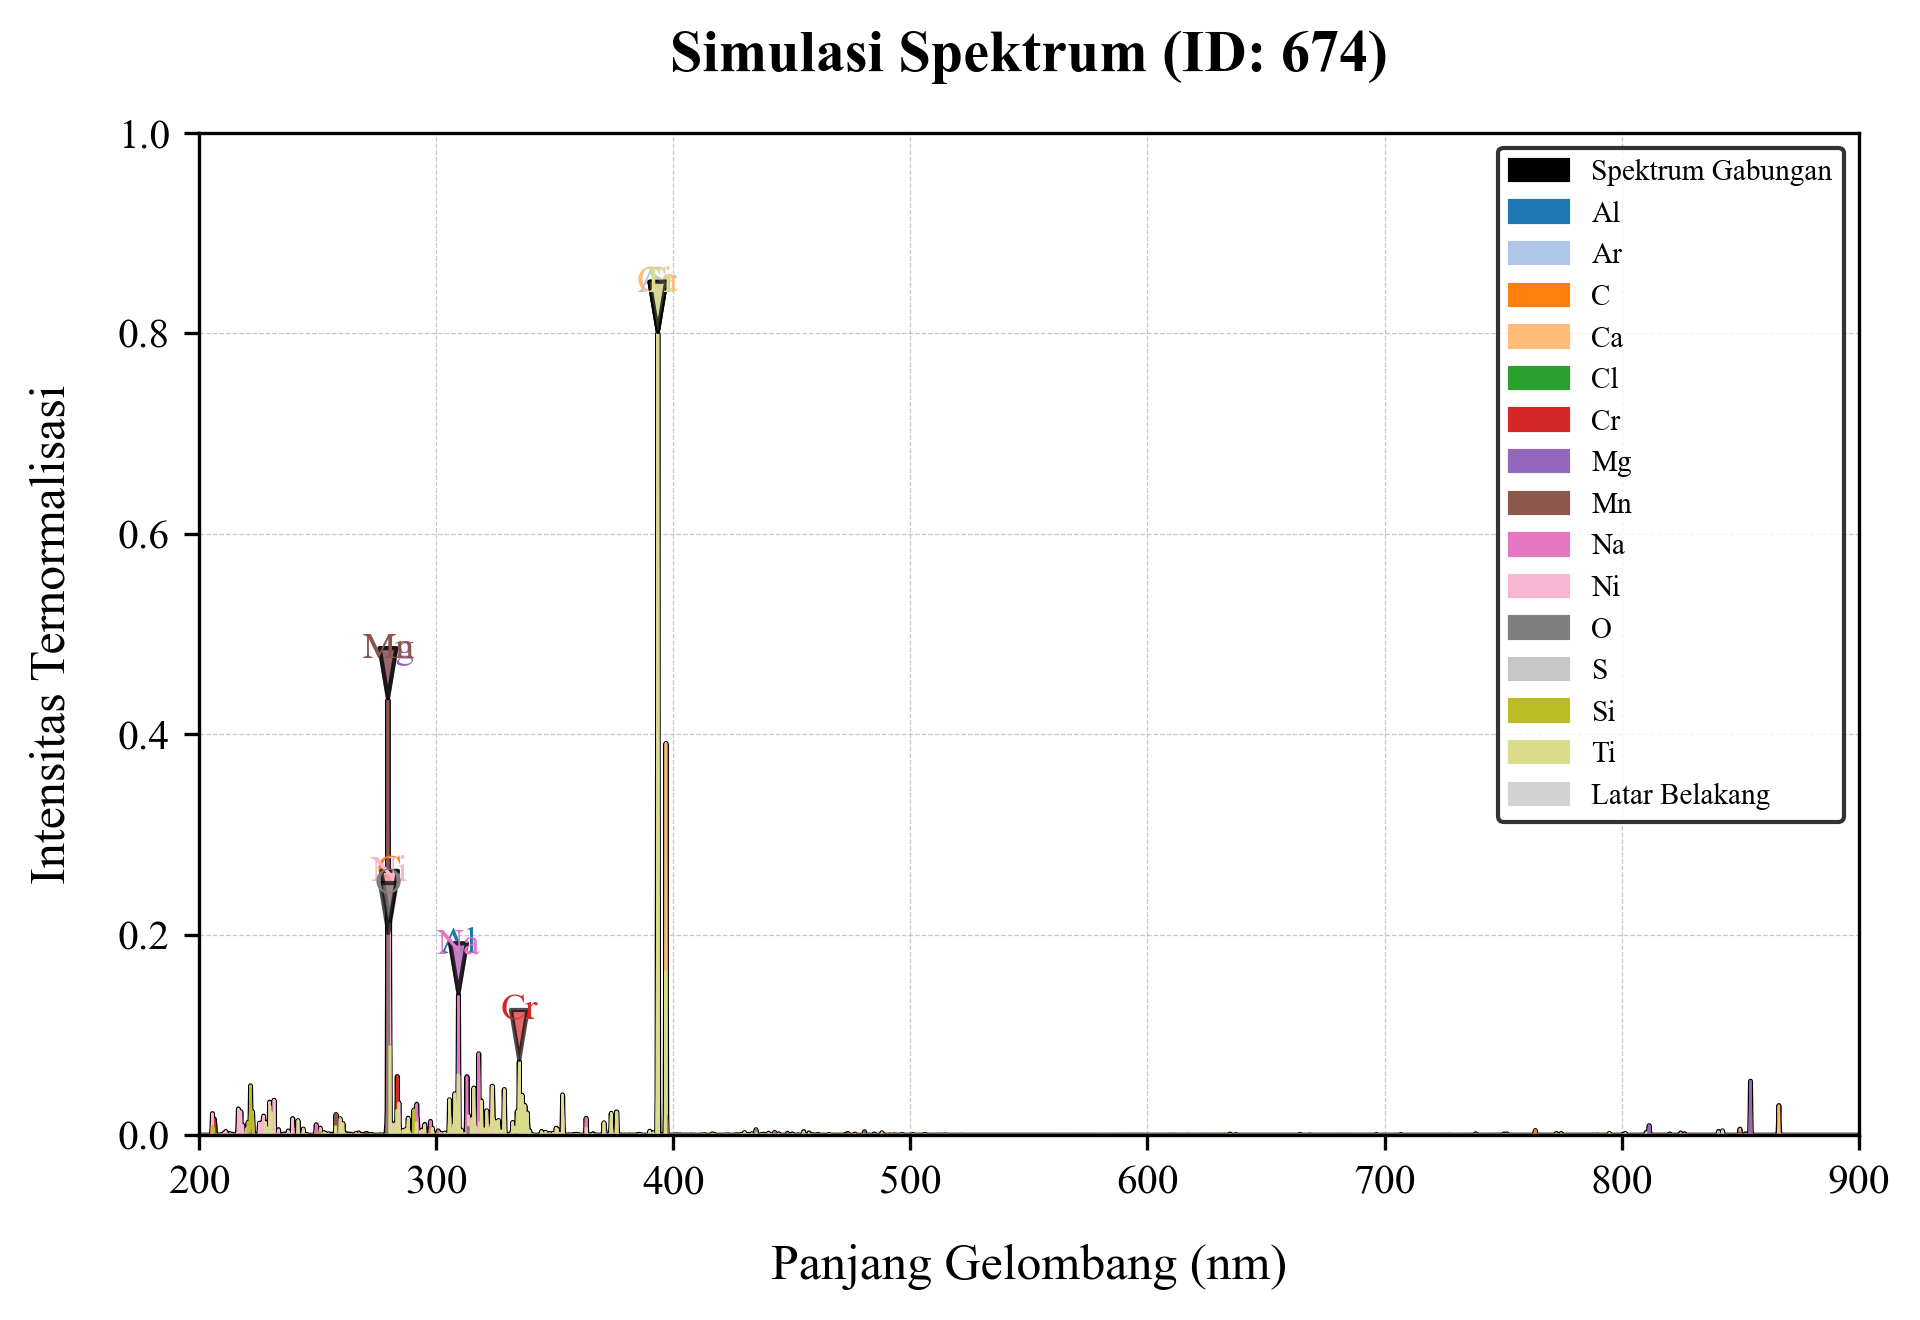
\includegraphics[width=1.2\textwidth, angle=90]{spectrum_674.png}
        \caption{Spectral simulation plot for sample 674 in full horizontal layout.}
        \label{fig:spectrum_674}
    \end{landscape}
\end{figure}

\clearpage

\section{Sample: 1636}
\subsection{Simulation Parameters}
\begin{table}[h!]
    \centering
    \begin{tabular}{ll}
        \toprule
        \textbf{Parameter} & \textbf{Value} \\
        \midrule
        Temperature ($T$) & 8737 \,\si{K} \\
        Electron Density ($n_e$) & 2.48e+17 \,\si{cm^-3} \\
        Total Pixels & 4096 \\
        Signal-to-Noise Ratio (SNR) & 32.07 \\
        \bottomrule
    \end{tabular}
    \caption{Simulation parameters and additional metrics for sample 1636.}
    \label{tab:params_1636}
\end{table}

\subsection{Composition Analysis}
\begin{table}[h!]
    \centering
    \begin{tabular}{lcc}
        \toprule
        \textbf{Element} & \textbf{Initial Composition (\%)} & \textbf{Actual Positions} \\
        \midrule
        Al & 9.88 & 424.0 \\
        Ar & 0.78 & 629.0 \\
        C & 3.36 & 222.0 \\
        Ca & 10.11 & 150.0 \\
        Cl & 3.55 & 12.0 \\
        Co & 0.52 & 1371.0 \\
        Cr & 2.84 & 397.0 \\
        Fe & 0.00 & 0.0 \\
        Mg & 10.17 & 346.0 \\
        Mn & 0.87 & 706.0 \\
        N & 7.93 & 396.0 \\
        Na & 11.72 & 330.0 \\
        Ni & 4.95 & 478.0 \\
        O & 14.61 & 170.0 \\
        S & 7.11 & 68.0 \\
        Si & 7.37 & 218.0 \\
        Ti & 4.23 & 1183.0 \\
        background & N/A & 797.0 \\

        \midrule
        \textbf{Total Positions} & & 7897.0 \\
        \bottomrule
    \end{tabular}
    \caption{Composition analysis for sample 1636.}
    \label{tab:comp_1636}
\end{table}

\subsection{Spectral Plot}
\begin{figure}[p]
    \begin{landscape}
        \centering
        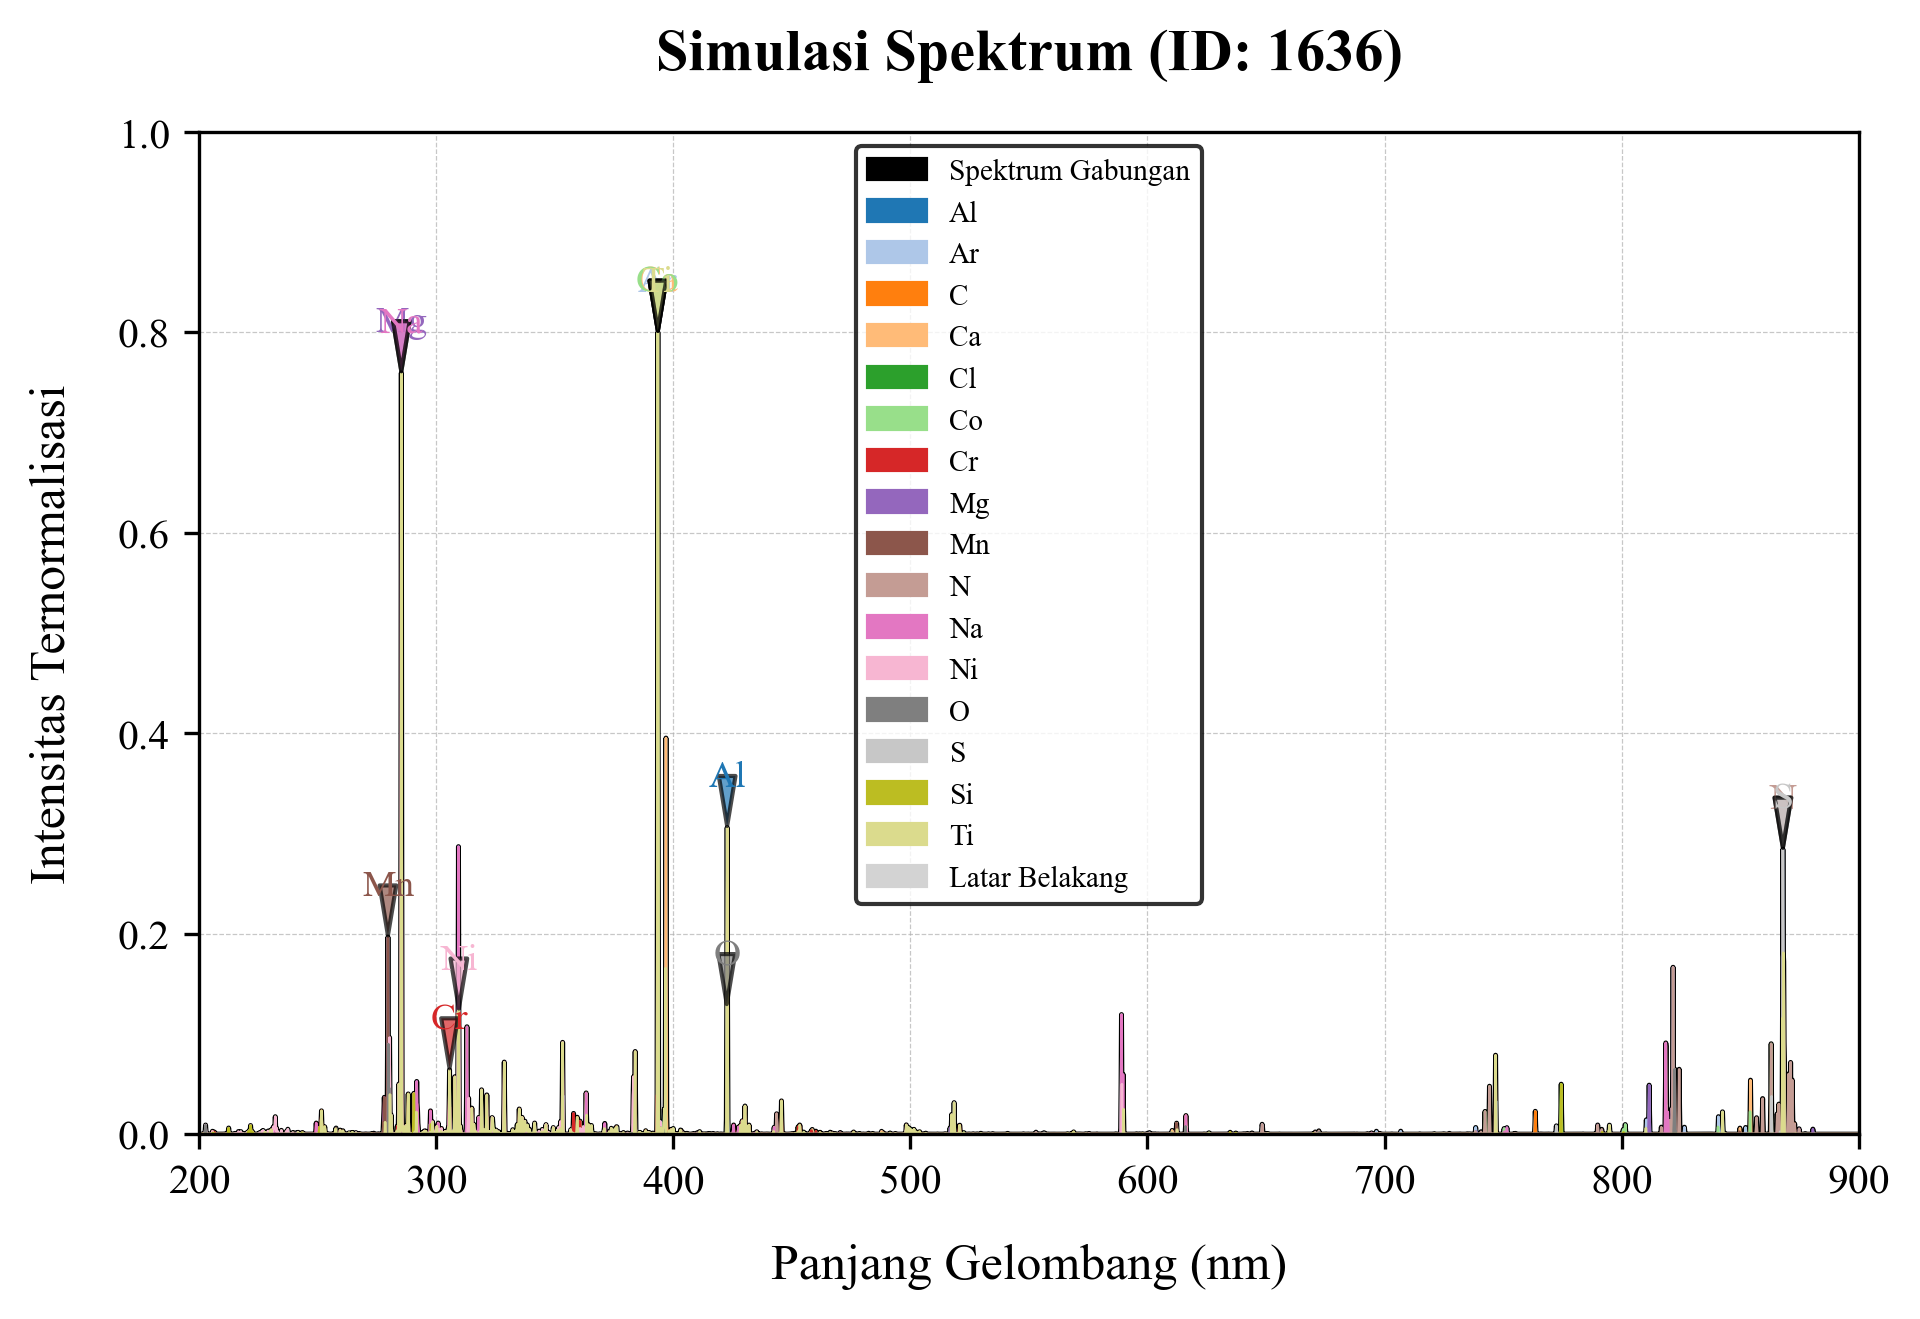
\includegraphics[width=1.2\textwidth, angle=90]{spectrum_1636.png}
        \caption{Spectral simulation plot for sample 1636 in full horizontal layout.}
        \label{fig:spectrum_1636}
    \end{landscape}
\end{figure}

\clearpage

\end{document}
